\documentclass[12pt,titlepage]{article}
\usepackage[margin=1.25in]{geometry}
\usepackage{graphicx,amsmath,blindtext,minted}

%% Variables definition
\newcommand{\vSubject}{Data Structure and Algorithm Practicum}
\newcommand{\vSubtitle}{Array of Objects}
\newcommand{\vName}{Dicha Zelianivan Arkana}
\newcommand{\vNIM}{2241720002}
\newcommand{\vClass}{1i}
\newcommand{\vDepartment}{Information Technology}
\newcommand{\vStudyProgram}{D4 Informatics Engineering}

%% [START] Tikz related stuff
\usepackage{tikz}
\usetikzlibrary{svg.path,calc,shapes.geometric,shapes.misc}
\tikzstyle{terminator} = [rectangle, draw, text centered, rounded corners = 1em, minimum height=2em]
\tikzstyle{preparation} = [chamfered rectangle, chamfered rectangle sep=0.75em, draw, text centered, minimum height = 2em]
\tikzstyle{process} = [rectangle, draw, text centered, minimum height=2em]
\tikzstyle{decision} = [diamond, aspect=2, draw, text centered, minimum height=2em]
\tikzstyle{data}=[trapezium, draw, text centered, trapezium left angle=60, trapezium right angle=120, minimum height=2em]
\tikzstyle{connector} = [line width=0.25mm,->]
%% [END] Tikz related stuff

%% [START] Fancy header related stuff
\usepackage{fancyhdr}
\pagestyle{fancy}
\setlength{\headheight}{15pt} % compensate fancyhdr style
\fancyhead{}
\fancyfoot{}
\fancyfoot[L]{\thepage}
\fancyfoot[R]{\textit{\vSubject - \vSubtitle}}
\renewcommand{\footrulewidth}{0.4pt}% default is 0pt, overline for footer
%% [END] Fancy header related stuff

%% [START] Custom tabular command related stuff
\usepackage{tabularx}
\newcommand{\details}[2]{
    #1 & #2  \\
}
%% [END] Custom tabular command related stuff

%% [START] Figure related stuff
\newcommand{\image}[3][1]{
    \begin{figure}[h]
        \centering
        \includegraphics[#1]{#2}
        \caption{#3}
        \label{#3}
    \end{figure}
}
%% [END] Figure related stuff

\begin{document}
\begin{titlepage}
    \centering
    \vfill
    {\bfseries\LARGE
        \vSubject\\
        \vskip0.25cm
        \vSubtitle
    }
    \vfill
    
\includegraphics[width=6cm]{images/polinema-logo.png}
    \vfill
    {
        \textbf{Name}\\
        \vName\\
        \vskip0.5cm
        \textbf{NIM}\\
        \vNIM\\
        \vskip0.5cm
        \textbf{Class}\\
        \vClass\\
        \vskip0.5cm
        \textbf{Department}\\
        \vDepartment\\
        \vskip0.5cm
        \textbf{Study Program}\\
        \vStudyProgram
    }
\end{titlepage}

\tableofcontents

\newpage2

\setcounter{section}{1}
\setcounter{subsection}{1}

\subsection{Create, insert, and display Array of Object}
\subsubsection{Steps}
\begin{enumerate}
    \item Create a new project with name ArrayOfObjects. Create the package with name ‘week3’
    \item {
        Create a \textbf{Rectangle} class:

        \begin{minted}[autogobble,fontsize=\small]{java}
            public class Rectangle {
                public int length;
                public int width;
            }
        \end{minted}
    }
    \item {
        In main method in ArrayOfObjects class, create an array Rectangle and its length is 3

        \begin{minted}[autogobble,fontsize=\small]{java}
            public class ArrayOfObjects {
                public static void main(String[] args) {
                    Rectangle[] rectangleArray = new Rectangle[3];
                }
            }
        \end{minted}
    }
    \item {
        Then insert values for each of the object's attributes

        \begin{minted}[autogobble,fontsize=\small]{java}
            rectangleArray[0] = new Rectangle();
            rectangleArray[0].length = 110;
            rectangleArray[0].width = 30;

            rectangleArray[1] = new Rectangle();
            rectangleArray[1].length = 80;
            rectangleArray[1].width = 40;

            rectangleArray[2] = new Rectangle();
            rectangleArray[2].length = 100;
            rectangleArray[2].width = 20;
        \end{minted}
    }
    \item {
        Print all the attributes object from ppArray as follows

        \begin{minted}[autogobble,fontsize=\small]{java}
            System.out.println("First rectangle, width: " + rectangleArray[0].width + ", length: " + rectangleArray[0].length);
            System.out.println("Second rectangle, width: " + rectangleArray[1].width + ", length: " + rectangleArray[1].length);
            System.out.println("Third rectangle, width: " + rectangleArray[2].width + ", length: " + rectangleArray[2].length);
        \end{minted}
    }
\end{enumerate}

\newpage

\subsubsection{Result}
Compile the code and see the result if it matches with the following image.

\begin{figure}[h]
    \centering
    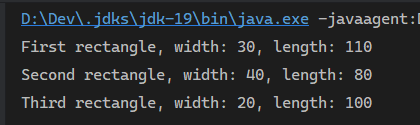
\includegraphics[width=12cm]{./images/array-of-objects.png}
    \caption{The result}
\end{figure}

\subsubsection{Questions}
\begin{enumerate}
    \item {
        An object used for the array is not required to have both attribute \textit{and} method.
        It needs to have either one of them, or both, but it depends on the use case. If we do need the attribute then we add it,
        if we don't need it then we don't have to add it.

        In this case specifically, we need the attributes for the rectangle because an object without attribute or method would be useless.
    }
    \item {
        Every class in java, if we don't define the constructor, we can use the parameterless constructor adding it explicitly.
    }
    \item {
        We initialise an array of \texttt{Rectangle} with the length of 3
    }
    \item {
        We set the first element of the array \texttt{rectangleArray} with an instance of Rectangle,
        and we set the \texttt{length} and \texttt{width} attribute with a number
    }
    \item {
        It is not required, but it's better if we differentiate them to better modularise our code
        and apply the Single Responsibility Principle which means that a class should only concern about one thing
        and one thing only.
    }
\end{enumerate}

\subsection{Get input in array of Objects using Loops}
\subsubsection{Questions}
\begin{enumerate}
    \item {
        The array of objects can be implemented on 2D array.
        We would write it like how we would write it normally with primitive datatype.
    }
    \newpage
    \item {
        Example of 2D array using objects:

        \begin{minted}[autogobble,fontsize=\small]{java}
            Point[][] coordinates = new Point[10][2];
        \end{minted}
    }
    \item {
        Because we haven't instantiated the array but we try to change its attribute value.
    }
    \item {
        \begin{minted}[autogobble,fontsize=\small]{java}
            import java.util.Scanner;

            public class ArrayOfObjects {
                public static void main(String[] args) {
                    Scanner sc = new Scanner(System.in);

                    System.out.print("Insert the length of the array: ");
                    int length = sc.nextInt();

                    Rectangle[] rectangleArray = new Rectangle[length];

                    for (int i = 0; i < length; i++) {
                        rectangleArray[i] = new Rectangle();
                        System.out.println("Rectangle " + i);

                        System.out.print("Input length: ");
                        rectangleArray[i].length = sc.nextInt();

                        System.out.print("Input width: ");
                        rectangleArray[i].width = sc.nextInt();
                    }

                    for (int i = 0; i < length; i++) {
                        System.out.println("Rectangle " + i);
                        System.out.println("width: " + rectangleArray[0].width + ", length: " + rectangleArray[0].length);
                    }
                }
            }
        \end{minted}
    }
    \item {
        Yes, if we do that then the previous value will get overriden
    }
\end{enumerate}

\subsection{Mathematical operation in array of object's attribute}
\subsubsection{Questions}
\begin{enumerate}
    \item {
        Yes, we can have multiple constructors in a single class as long as they have different signatures.
        It's called "overloading"
    }
    \newpage
    \item {
        Create a Triangle class

        \begin{minted}[autogobble,fontsize=\small]{java}
            public class Triangle {
                public int base;
                public int height;
            }
        \end{minted}
    }
    \item {
        \begin{minted}[autogobble,fontsize=\small]{java}
            public class Triangle {
                public int base;
                public int height;

                public Triangle(int a, int t) {
                    this.base = a;
                    this.height = t;
                }

                public double calculateArea() {
                    return (double)(base/2)*height;
                }

                public double calculatePerimeter() {
                    double side = Math.sqrt(Math.pow(base, 2) + Math.pow(height, 2));
                    return side + base + height;
                }
            }
        \end{minted}
    }
    \item {
        \begin{minted}[autogobble,fontsize=\small]{java}
                public class TriangleMain {
                    public static void main(String[] args) {
                        Triangle[] triangles = new Triangle[4];

                        triangles[0] = new Triangle(10, 4);
                        triangles[1] = new Triangle(20, 10);
                        triangles[2] = new Triangle(15, 6);
                        triangles[3] = new Triangle(25, 10);
                    }
                }
        \end{minted}
    }
    \newpage
    \item {
        \begin{minted}[autogobble,fontsize=\small]{java}
            public class TriangleMain {
                public static void main(String[] args) {
                    Triangle[] triangles = new Triangle[4];

                    triangles[0] = new Triangle(10, 4);
                    triangles[1] = new Triangle(20, 10);
                    triangles[2] = new Triangle(15, 6);
                    triangles[3] = new Triangle(25, 10);

                    for (int i = 0; i < triangles.length; i++) {
                        Triangle triangle = triangles[i];
                        System.out.printf(
                                "%d. Area: %.2f | Perimeter: %.2f\n",
                                i + 1,
                                triangle.calculateArea(),
                                triangle.calculatePerimeter());
                    }
                }
            }
        \end{minted}

        \begin{figure}[h]
            \centering
            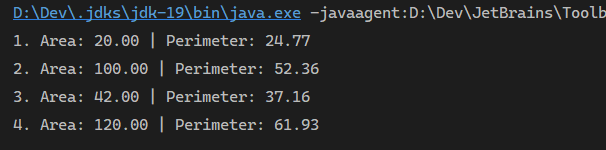
\includegraphics[width=13cm]{./images/triangles-output.png}
        \end{figure}
    }
\end{enumerate}
\newpage

\subsection{Practice}
\begin{enumerate}
    \item {
        \textbf{Cube.java}
        \begin{minted}[autogobble,fontsize=\small]{java}
            public class Cube {
                public int vertice;

                public double calculateVolume() {
                    return Math.pow(vertice, 3);
                }

                public double calculateSurfaceArea() {
                    return vertice * vertice * 12;
                }
            }
        \end{minted}

        \newpage

        \textbf{CubeMain.java}
        \begin{minted}[autogobble,fontsize=\small]{java}
            import java.util.Scanner;

            public class CubeMain {
                public static void main(String[] args) {
                    Scanner input = new Scanner(System.in);

                    System.out.print("Insert the limit: ");
                    int limit = input.nextInt();
                    Cube[] cubes = new Cube[limit];

                    for (int i = 0; i < cubes.length; i++) {
                        cubes[i] = new Cube();
                        System.out.printf("%d. Insert the vertice length: ", i + 1);
                        cubes[i].vertice = input.nextInt();
                    }

                    for (int i = 0; i < cubes.length; i++) {
                        System.out.printf(
                                "%d. Surface Area: %.2f | Volume: %.2f\n",
                                i + 1,
                                cubes[i].calculateSurfaceArea(),
                                cubes[i].calculateVolume()
                        );
                    }
                }
            }
        \end{minted}

        \begin{figure}[h]
            \centering
            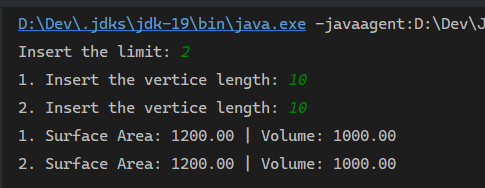
\includegraphics[width=13cm]{./images/3d-shapes.png}
        \end{figure}
    }
    \newpage
    \item {
        \begin{minted}[autogobble,fontsize=\small]{java}
            import java.util.Scanner;

            public class LandMain {
                public static void main(String[] args) {
                    Scanner input = new Scanner(System.in);

                    System.out.print("How many lands? ");
                    int limit = input.nextInt();

                    Land[] lands = new Land[limit];
                    for (int i = 0; i < lands.length; i++) {
                        lands[i] = new Land();
                        System.out.printf("Land %d\n", i + 1);
                        System.out.print("Length: ");
                        lands[i].length = input.nextInt();
                        System.out.print("Width: ");
                        lands[i].width = input.nextInt();
                    }

                    for (int i = 0; i < lands.length; i++) {
                        System.out.printf(
                            "Land Area %d: %.2f\n", 
                            i + 1, lands[i].calculateArea()
                        );
                    }
                }
            }
        \end{minted}
    }
    \item {
        \begin{minted}[autogobble,fontsize=\small]{java}
            import java.util.Scanner;

            public class LandMain {
                static void printWidestArea(Land[] lands) {
                    int widestIndex = 0;
                    for (int i = 1; i < lands.length; i++) {
                        if (lands[i].calculateArea() > lands[widestIndex].calculateArea()) {
                            widestIndex = i;
                        }
                    }
                    System.out.printf("The widest land is Land %d", widestIndex);
                }
                
                public static void main(String[] args) {
                    Scanner input = new Scanner(System.in);

                    System.out.print("How many lands? ");
                    int limit = input.nextInt();

                    Land[] lands = new Land[limit];
                    for (int i = 0; i < lands.length; i++) {
                        lands[i] = new Land();
                        System.out.printf("Land %d\n", i + 1);
                        System.out.print("Length: ");
                        lands[i].length = input.nextInt();
                        System.out.print("Width: ");
                        lands[i].width = input.nextInt();
                    }

                    for (int i = 0; i < lands.length; i++) {
                        System.out.printf("Land Area %d: %.2f\n", i + 1, lands[i].calculateArea());
                    }

                    System.out.println();
                    printWidestArea(lands);
                }
            }

        \end{minted}
    }
    \item {
        \begin{minted}[autogobble,fontsize=\small]{java}
            public class Student {
                public String name;
                public String nim;
                public char gender;
                public double ipk;
            }
        \end{minted}

        \begin{minted}[autogobble,fontsize=\small]{java}
            import java.util.Scanner;

            public class StudentMain {
                static void printAverageScore(Student[] students) {
                    double total = 0;
                    for (Student student : students) {
                        total += student.ipk;
                    }
                    System.out.printf("Average IPK of all students : %.2f", total / students.length);
                }

                public static void main(String[] args) {
                    Scanner input = new Scanner(System.in);

                    System.out.println("Insert the limit: ");
                    int limit = input.nextInt();
                    Student[] students = new Student[limit];

                    for (int i = 0; i < students.length; i++) {
                        System.out.print("Insert name: ");
                        students[i].name = input.next();
                        System.out.print("Insert nim: ");
                        students[i].nim = input.next();
                        System.out.print("Insert gender: ");
                        students[i].gender = input.next().charAt(0);
                        System.out.print("Insert ipk: ");
                        students[i].ipk = input.nextDouble();
                    }

                    for (int i = 0; i < students.length; i++) {
                        System.out.printf(
                                "Student %d\nname : %s\nnim : %s\ngender : %c\nIPK score : %.2f\n\n",
                                i + 1,
                                students[i].name,
                                students[i].nim,
                                students[i].gender,
                                students[i].ipk
                        );
                    }
                }
            }

        \end{minted}
    }
    \item {
        \begin{minted}[autogobble,fontsize=\small]{java}
            import java.util.Scanner;

            public class StudentMain {
                static void printAverageScore(Student[] students) {
                    double total = 0;
                    for (Student student : students) {
                        total += student.ipk;
                    }
                    System.out.printf("Average IPK of all students : %.2f", total / students.length);
                }

                public static void main(String[] args) {
                    Scanner input = new Scanner(System.in);

                    System.out.println("Insert the limit: ");
                    int limit = input.nextInt();
                    Student[] students = new Student[limit];

                    for (int i = 0; i < students.length; i++) {
                        System.out.print("Insert name: ");
                        students[i].name = input.next();
                        System.out.print("Insert nim: ");
                        students[i].nim = input.next();
                        System.out.print("Insert gender: ");
                        students[i].gender = input.next().charAt(0);
                        System.out.print("Insert ipk: ");
                        students[i].ipk = input.nextDouble();
                    }

                    for (int i = 0; i < students.length; i++) {
                        System.out.printf(
                                "Student %d\nname : %s\nnim : %s\ngender : %c\nIPK score : %.2f\n\n",
                                i + 1,
                                students[i].name,
                                students[i].nim,
                                students[i].gender,
                                students[i].ipk
                        );
                    }
                }
            }

        \end{minted}
    }
\end{enumerate}

\end{document}

